%!TEX program = xelatex
%Template created by: Maciej Byczko
\documentclass[a4paper,12pt]{extarticle}  %typ dokumentu

\usepackage[utf8]{inputenc} %rodzaj czcionki w dokumencie
\usepackage{geometry} %poprawienie marginesów
\usepackage{polski} %polskie znaki
\usepackage{multirow} %tabela
\usepackage{graphicx} %tabela
\usepackage{float} %poprawienie pozycji
\usepackage{fancyhdr} % header i footer
\usepackage{karnaugh-map} % rysowanie siatek karnaugh
\usepackage{hyperref} %tworzenie odnośników, \url{<url>}, \href{<file path, link>}{<text with link>} \pageref{}
\usepackage{amsmath} % Matma
\usepackage{boldline}%edytowanie grubości krawędzi w tabelach \hlineB{} \clineB{}{}
\usepackage{array}%grubsze kolumny w tabeli
\usepackage{bigstrut}
\usepackage{caption}
%Ustawienie paczki hyperref
\hypersetup{
     colorlinks,
     citecolor=black,
     filecolor=black,
     linkcolor=black,
     urlcolor=black
}
\graphicspath{{pictures/}}
\geometry{margin=0.7in}
\pagestyle{fancy}

% (fancyhdr)	You might also make \topmargin smaller to compensate:

\cfoot{Strona \thepage}
\rhead{Strona \thepage}
\lhead{\typdoc}
\newcolumntype{?}{!{\vrule width 1.5pt}}

\title{\tytul}
\author{\tworcy}
\date{\data}

%-----------------------PRZYDATNE LINKI----------------------------------
%link do tworzenia tabeli https://tablesgenerator.com
%symbole matematyczne: https://oeis.org/wiki/List_of_LaTeX_mathematical_symbols
%narzędzia matematyczne: https://en.wikibooks.org/wiki/LaTeX/Mathematics
%krótkie podpowiedzi http://www.mif.pg.gda.pl/homepages/sylas/students/wdi/doc/latex-sciaga.html
%symbole do schematów: http://texdoc.net/texmf-dist/doc/latex/circuitikz/circuitikzmanual.pdf
%----------------------------------------------------------------------

%-----------------------SEKCJA DANYCH----------------------------------
\def\tytul{Układy Kombinacyjne} %<<< tytuł ćwiczenia
\def\nrcw{2} %<<< numer ćwiczenia
\def\data{10 Października 2021} %<< data wykonania
\def\prowadzacy{dr inż. Jacek Mazurkiewicz} %<<<prowadzący
\def\nrgrupy{B} %<<<numer grupy
\def\tworcy{Maciej Byczko\\Bartosz Matysiak} %<<< autorzy
\def\zajinfo{PN 10:50 TP} %<<< informacje dotyczące zajęć
\def\typdoc{Sprawozdanie} %<<< typ dokumentu tj Sprawozdanie, zadania itp. {Matematyka dyskretna/Sprawozdanie z Miernictwa}
% \tableofcontents % Stworzenie spis treści
%JEŻELI COS JESZCZE POTRZEBA W TEJ SEKCJI TO POINFORMOWAĆ!!!
%----------------------------------------------------------------------

%-----------------------SEKCJA FORMATOWANIA----------------------------
% \textbf{pogrubienie}  \textit{kursywa}    \underline{podkreślenie}
% \vspace*{2mm} - Odstęp pionowy między tekstem
%----------------------------------------------------------------------

\begin{document}
\setlength{\headheight}{15pt}

%-------------------------------------TABELA-DANYCH--------------------------------------------------
\begin{table}[H]
	\centering
	\resizebox{\textwidth}{!}{
		\begin{tabular}{|c|c|c|}\hline
			\begin{tabular}[c]{@{}c@{}}                     \tworcy     \end{tabular} &
			\begin{tabular}[c]{@{}c@{}}Prowadzący:\\        \prowadzacy \end{tabular} &
			\begin{tabular}[c]{@{}c@{}}Numer ćwiczenia\\    \nrcw       \end{tabular}          \\ \hline
			\begin{tabular}[c]{@{}c@{}}                     \zajinfo    \end{tabular} &
			\begin{tabular}[c]{@{}c@{}}Temat ćwiczenia:\\   \tytul      \end{tabular} & Ocena: \\ \hline
			\begin{tabular}[c]{@{}c@{}}Grupa:\\          \nrgrupy    \end{tabular}    &
			\begin{tabular}[c]{@{}c@{}}Data wykonania:\\    \data       \end{tabular} &        \\ \hline
		\end{tabular}}
\end{table}
%----------------------------------------------------------------------------------------------------
\tableofcontents
\cleardoublepage
\section{Zadanie 1}
\subsection{Polecenie}
Wykonać dowolną bramkę - funktor: 2 wejścia, 1 wyjście
\subsection{Rozwiązanie}
\subsubsection{Schemat układu}
\begin{figure}[H]
   \centering
   \resizebox*{\textwidth}{!}{
	  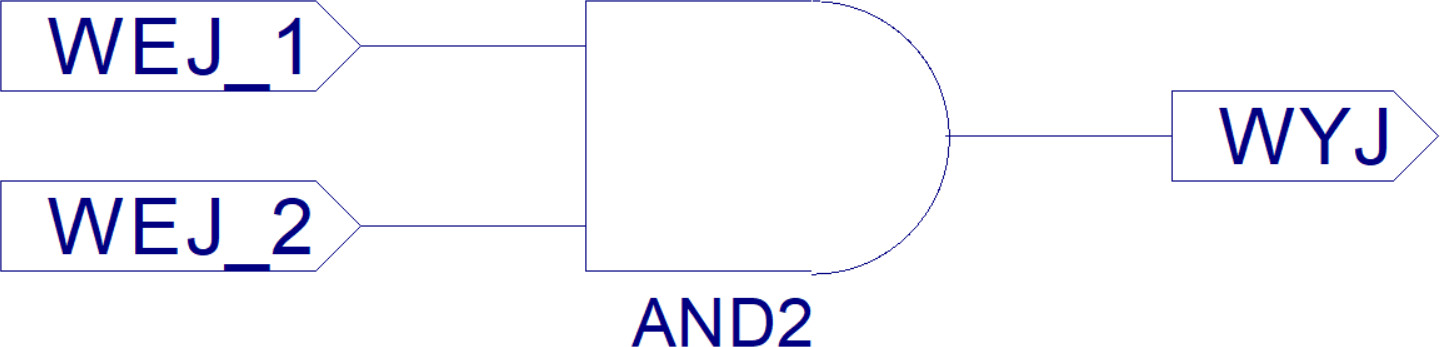
\includegraphics{schemat-zad1.png}
   }
\end{figure}

% screen z Xilinxa lub poszukać opcji eksportu grafiki
\subsubsection{Kod VHDL}
% tutaj użyjemy listing do wczytania pliku z kodem \lstinputlisting{}
\subsubsection{Symulacja}
% to samo co ze schematem lecz tytułowa symulacja
\section{Zadanie 2}
\subsection{Polecenie}
Implementacja funkcji logicznej \textbf{$G(w,x,y,z) = \prod(0, 2, 3, 4, 6, 7, 9, 11, 12, 13, 15)$}
\subsection{Rozwiązanie}
\subsubsection{Wyprowadzenie}
\begin{align}
	  & G(w,x,y,z) = \prod(0, 2, 3, 4, 6, 7, 9, 11, 12, 13, 15)                                                       \\
	= & \sum(1,5,8,14) = \sum(0001, 0101, 1000, 1010, 1110)                                                           \\
	= & \overline{wxy}z + \overline{w}x\overline{y}z + w\overline{xyz} + w\overline{x}y\overline{z} + wxy\overline{z} \\
	= & \overline{wy}z(\overline{x} + x) + w\overline{z}(\overline{xy} + \overline{x}y + xy)                          \\
	= & \overline{wy}z + w\overline{z}(\overline{x}(\overline{y} + y) + xy)                                           \\
	= & \overline{wy}z + w\overline{z}(\overline{x} + xy)                                                             \\
	= & \overline{wy}z + w\overline{z}((\overline{x} + x)(\overline{x} + y))                                          \\
	= & \overline{wy}z + w\overline{z}((\overline{x} + y))                                                            \\
	= & \overline{wy}z + w\overline{xz} + w\overline{z}y
\end{align}
\subsubsection{Tabela prawdy}
\begin{table}[H]
	\centering
	\resizebox{0.5\textwidth}{!}{
		\begin{tabular}{?c?c|c|c|c?c?}\hlineB{2.5}
			Kod dziesiętny & w & x & y & z & S \bigstrut \\\hlineB{2.5}
			0              & 0 & 0 & 0 & 0 & 0 \bigstrut \\\hline
			1              & 0 & 0 & 0 & 1 & 1 \bigstrut \\\hline
			2              & 0 & 0 & 1 & 0 & 0 \bigstrut \\\hline
			3              & 0 & 0 & 1 & 1 & 0 \bigstrut \\\hline
			4              & 0 & 1 & 0 & 0 & 0 \bigstrut \\\hline
			5              & 0 & 1 & 0 & 1 & 1 \bigstrut \\\hline
			6              & 0 & 1 & 1 & 0 & 0 \bigstrut \\\hline
			7              & 0 & 1 & 1 & 1 & 0 \bigstrut \\\hline
			8              & 1 & 0 & 0 & 0 & 1 \bigstrut \\\hline
			9              & 1 & 0 & 0 & 1 & 0 \bigstrut \\\hline
			10             & 1 & 0 & 1 & 0 & 1 \bigstrut \\\hline
			11             & 1 & 0 & 1 & 1 & 0 \bigstrut \\\hline
			12             & 1 & 1 & 0 & 0 & 0 \bigstrut \\\hline
			13             & 1 & 1 & 0 & 1 & 0 \bigstrut \\\hline
			14             & 1 & 1 & 1 & 0 & 1 \bigstrut \\\hline
			15             & 1 & 1 & 1 & 1 & 0 \bigstrut \\\hlineB{2.5}
		\end{tabular}%
	}
	\label{zad2-TableTrue}%
\end{table}%
\subsection{Siatka Karnaugh}
\begin{center}

\resizebox{0.5\textwidth}{!}{
	\begin{karnaugh-map}[4][4][1][$wx$][$yz$]
	\minterms{2,4,5,10,11} % na tych koordynatach umieść jedynki (1)
	\autoterms[0] % umieść ten symbol w miejscach niezdefiniowanych
	% \maxterms{0,1,3,6,7,8,9,12,13,14,15} % na tych koordynatach umieść zera (0)
	% \indeterminants{2,5} 
	% \implicant{3}{2}
	\implicant{4}{5} % połącz te komórki
	\implicant{11}{10}
	\implicantedge{2}{2}{10}{10} %połącz komórki brzegowe
	\end{karnaugh-map}
}
\end{center}
Równanie po minimalizacji: $w\overline{x}\overline{z} + \overline{w}\overline{y}z + wy\overline{z}$
\subsubsection{Schemat układu}
% screen z Xilinxa lub poszukać opcji eksportu grafiki
\subsubsection{Kod VHDL}
% tutaj użyjemy listing do wczytania pliku z kodem \lstinputlisting{}
\subsubsection{Symulacja}
% to samo co ze schematem lecz tytułowa symulacja
\section{Zadanie 3}
\subsection{Polecenie}
Implementacja układu translatora kodu \textbf{4-bit kod NKB na 4-bit kod Aikena}
\subsection{Rozwiązanie}
\subsubsection{Tabela Prawdy}
\begin{table}[H]
	\centering
	% \caption{Add caption}
	\resizebox{0.5\textwidth}{!}{
		\begin{tabular}{?c?c|c|c|c?c|c|c|c?}\hlineB{2.5}
			\multirow{2}[4]{*}{Kod dziesiętny} & \multicolumn{4}{c?}{NKB} & \multicolumn{4}{c?}{Kod Ikena} \bigstrut                                   \\\clineB{2-9}{2.5}
			                                   & w                        & x                                        & y & z & w & x & y & z \bigstrut \\\hlineB{2.5}
			0                                  & 0                        & 0                                        & 0 & 0 & 0 & 0 & 0 & 0 \bigstrut \\\hline
			1                                  & 0                        & 0                                        & 0 & 1 & 0 & 0 & 0 & 1 \bigstrut \\\hline
			2                                  & 0                        & 0                                        & 1 & 0 & 0 & 0 & 1 & 0 \bigstrut \\\hline
			3                                  & 0                        & 0                                        & 1 & 1 & 0 & 0 & 1 & 1 \bigstrut \\\hline
			4                                  & 0                        & 1                                        & 0 & 0 & 0 & 1 & 0 & 0 \bigstrut \\\hline
			5                                  & 0                        & 1                                        & 0 & 1 & 1 & 0 & 1 & 1 \bigstrut \\\hline
			6                                  & 0                        & 1                                        & 1 & 0 & 1 & 1 & 0 & 0 \bigstrut \\\hline
			7                                  & 0                        & 1                                        & 1 & 1 & 1 & 1 & 0 & 1 \bigstrut \\\hline
			8                                  & 1                        & 1                                        & 0 & 0 & 1 & 1 & 1 & 0 \bigstrut \\\hline
			9                                  & 1                        & 0                                        & 0 & 1 & 1 & 1 & 1 & 1 \bigstrut \\\hline
			10                                 & 1                        & 0                                        & 1 & 0 & - & - & - & - \bigstrut \\\hline
			11                                 & 1                        & 0                                        & 1 & 1 & - & - & - & - \bigstrut \\\hline
			12                                 & 1                        & 1                                        & 0 & 0 & - & - & - & - \bigstrut \\\hline
			13                                 & 1                        & 1                                        & 0 & 1 & - & - & - & - \bigstrut \\\hline
			14                                 & 1                        & 1                                        & 1 & 0 & - & - & - & - \bigstrut \\\hline
			15                                 & 1                        & 1                                        & 1 & 1 & - & - & - & - \bigstrut \\\hlineB{2.5}
		\end{tabular}%
	}
	\label{zad3-TableTrue}%
\end{table}%
\subsubsection{Siatki Karnaugh}
\begin{figure}[H]
\centering
\begin{minipage}[c]{0.4\linewidth}
\begin{karnaugh-map}[4][4][1][$wx$][$yz$]
\maxterms{0,1,2,3,4}
\minterms{5,6,7,8,9}
\implicant{12}{10}
\implicant{5}{15}
\implicant{7}{14}
\autoterms[-]
\end{karnaugh-map}
\caption*{$w = zx + zw + y$}
\end{minipage}
\begin{minipage}[c]{0.4\linewidth}
\begin{karnaugh-map}[4][4][1][$wx$][$yz$]
\maxterms{0,1,2,3,5}
\minterms{4,6,7,8,9}
\implicant{12}{10}
\implicant{7}{14}
\implicantedge{4}{12}{6}{14}
\autoterms[-]
\end{karnaugh-map}
\caption*{$x = z\overline{x} + zw + y$}
\end{minipage}
\end{figure}

\begin{figure}[H]
	\centering
\begin{minipage}[c]{0.4\linewidth}
\begin{karnaugh-map}[4][4][1][$wx$][$yz$]
\maxterms{0,1,4,6}
\minterms{2,3,5,7,8,9}
\implicant{12}{10}
\implicant{5}{15}
\implicantedge{3}{2}{11}{10}
\autoterms[-]
\end{karnaugh-map}
\caption*{$y = \overline{z}w + zx + y$}
\end{minipage}
\begin{minipage}[c]{0.4\linewidth}
\begin{karnaugh-map}[4][4][1][$wx$][$yz$]
\maxterms{0,2,4,6,8}
\minterms{1,3,5,7,9}
\implicant{1}{11}
\autoterms[-]
\end{karnaugh-map}
\caption*{$z = x$}
\end{minipage}

\end{figure}
\subsubsection{Schemat układu}
% screen z Xilinxa lub poszukać opcji eksportu grafiki
\subsubsection{Kod VHDL}
% tutaj użyjemy listing do wczytania pliku z kodem \lstinputlisting{}
\subsubsection{Symulacja}
% to samo co ze schematem lecz tytułowa symulacja
\section{Wnioski}

\end{document}